\documentclass[letter, 12pt, titlepage]{article}
\usepackage{graphicx}
\setlength{\parindent}{0pt}

\usepackage[left=1in,right=1in,top=1in,bottom=1in]{geometry}




\author{ Dispoto, Brett\\
        \and
        Kamel, Adham\\
        \and
        Cai, Feiyu\\
}


\title{CS157A Project Requirement Documentation \\
        \large A Book Reading and Review Web Application}

\begin{document}

  \maketitle
        \section{Project Overview}
        \subsection{Application Overview}
        Our team will be developing a database application where users can find free books and are able to download them via multiple formats and leave reviews on those books for other customers to see. The books that the user can see will be ranging from textbooks to novels. A user will be given the option to create an account, or if they already registered, login to their account. After this, the user will be able to search for a specific book, whether that is by the title of the book or its ISBN number. If the user does not know the specific book they want to find, they can search for a specific author, or genre. Searches will include various filtering options such as date published, publisher, book length, user favorites, etc. Users can sort search results by the title alphabetically, the author alphabetically, or by book rating.

\medskip
        In our application, users will be able to leave reviews on books that they have read, which will be seen by other users and possibly influence their decision on their book. These reviews will contain both a comment section and a star rating system. Users will be able to comment how they either liked or disliked the book and give a star rating from one to five. The average star rating and total number of reviews will be displayed next to the book. Users will also be able to share the book they like with others with a shareable link that they can distribute how they please.
	\subsection{Project Motivation}
	The motivation behind this project is that as college students, we find ourselves paying several hundreds of dollars on college textbooks alone every semester, only to have them sitting on a shelf afterwards not being opened. Those hundreds of dollars spent on semester long textbooks could have been better utilized for students on other needs such as groceries or rent. We want to make a website to give students that option, giving them a website where they can download their desired textbooks for free.
	\subsection{Project Goal}
	The Goal of this project is to provide a free and open source infrastructure where users can read books from the public domain. We wish to provide an easy-to-use ecosystem, which allows the user to read or review books with ease.
	\subsection{Benefits to Users}
	Users will have a community where they can \textbf{read and review books for free}. Right now, websites such as this exists, but they only serve one of the two main functionalities. Websites like gutenberg.org give the users access to free book repositiories, but do not allow for users to read and write reviews on books. Conversely, websites like bookpage.com provide reviews for books, but they are not open to the public, rather only a small number of selected reviwers. Our web application will take the best aspects of both these websites to provide the user an efficent solution for picking and reading online books for free.
    \subsection{Stakeholders and Importance}
    The stakeholders of our applications will be students who want to find free textbook alternative to the paid bookstore alternative, as well as casual and dedicated book readers who can find free books online and download them for instant reading. This application is important because it provides a streamlined way for book-readers to gain easy access to the books they want and get them in a timely manner.


	\section{System Environment}
	
			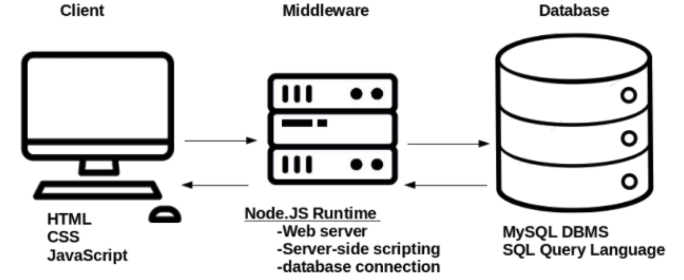
\includegraphics[scale=.66]{3-tier.png}
			\subsection{Presentation Layer}
			\begin{itemize}
			 \item HTML
				\begin{itemize}
					\item Purpose: HTML is the markup language supported by all major web-browsers. It allows content to be presented to a readable manner to the end-user. We will take advantage of HTML formatting tools such as hyperlinks, tables, and lists. Further, we will be using HTML forms for user input of email, username, password, search boxes, and comments.
					\item Version: HTML 5
				\end{itemize}
			\item Cascading Style Sheets (CSS)
			\begin{itemize}	
				\item Purpose: CSS will be used to improve the user experience of our web application. CSS gives us the ability to make animations, colored content, as well as more control of the appearance of our content.
				\item Version: CSS 3
			\end{itemize}
			\item	JavaScript (Client Side):
				\begin{itemize}
					\item	Purpose: Provide interactivity such as collection of user input, improve visual responsiveness, and sending alerts to users.
					\item Version: ECMA2016
				\end{itemize}
			\end{itemize}

		\subsection{Application Layer}
		\begin{itemize}
			\item Web Server: Node.js HTTP Module
			
				-Version: 10.6.3 LTS
			
			\item Server Side Application Language: JavaScript
				
				-Purpose: Provide communition between the presentation layer and the database layer
				-Version: EMCAScript2016

			\item	NPM Package Manger:

				-Purpose: Provide easy managment of external Node.js libraries such as express js, sql module, connect module, and http module.

				-Version: 6.9.0 
		\end{itemize}	
		\subsection{Data Layer}
		
			\begin{itemize}
			
			\item	This web application will require the use of a relational database management system (RDBMS), the specific RDBMS we will use is  MySQL.
			\item We will take advantage of the SQL programming language for tasks such as data definition, manipulation, query, control,and transaction control.
			\item MySQL RDBMS will take care of concurrency control, and will maintain the ACID principle for our database. 
			\item MySQL Version: 5.7.27
			\item Query Language: SQL
			\end{itemize}
		\subsection{Hardware/ Software Used}
		
		\begin{itemize}

			\item Client Software Requirements
			\begin{itemize}
				\item A web browser supporting the following is required to run the web application:
					\begin{itemize}
						\item ECMAScript2016
						\item HTML5
						\item CSS3
					\end{itemize}
			\item Since the 3-tier architecture will only be virtual, (no remote web server or DMBS), the client will be required to install the proper versions of Node.js as well as MySQL as specified. 
			
			\item  MySQL and Node.js are available on many operating systemssuch as Linux, MacOS, Microsoft Windows, FreeBSD, and OpenBSD	
			\end{itemize}

		\item Client Hardware Requirements:
			\begin{itemize}	
				\item Any hardware with support by the above software will be sufficient to run the web application.
			\end{itemize}
		\end{itemize}


\section{Functional Requirements}
		Because this application is to be accessed from a web browser, the \textbf{input} is a keyboard or mouse, while the \textbf{output} is stylized HTML to be displayed on a web browser. 

	\subsection{Comprehensive List of Features}
	\begin{itemize}

	\item	Search Book:
		\begin{itemize}
			\item  Users can search for books that on the system database
			\item  Input: ISBN, author, or title
			\item  Output: list of books that match with the input information
		\end{itemize}
	\item	Order Search Results:
		\begin{itemize}
			\item  User can order the book search results. Default search behavior is based on the number of favorites a book has received
			\item  Input: relese date or number of favorites
			\item  Output: ordered list of book that has characteristic from input
		\end{itemize}
	\item	Filter Search Results:
		\begin{itemize}
			\item  User can filter the search reslts 
			\item  Input: release date or genre
			\item  Output: filtered list of book that matched with characteristic from input
		\end{itemize}
	\item	Select Book:
		\begin{itemize}
			\item  Once user finds the desired book, they can select the book and view its profile.
			\item  Input: selecting single book
			\item  Output: book profile that includes book information and comments
		\end{itemize}
	\item	View Book Profile:


		A book's profile will consist of the following:
		\begin{itemize}
			\item The title of the book,
			\item The author,
			\item the relase date,
			\item the publisher,
			\item the ISBN,
			\item the reviews/comments left for the book,
			\item the number of "favorites" the book has received
		\end{itemize}
	\item Read/Download Book:
		\begin{itemize}
			\item  User can download the book and view it in their web browser.
			\item  Input: selecting single book
			\item  Ouput: reading page or download to local
		\end{itemize}
	\item Add/delete book to/from favorites:
		\begin{itemize}
			\item  Use can add the list to their "favorites", indicating that they enjoyed the book
			\item  Input: selecting single book
			\item  Output: add/delete book to/from the favorited book list that can be viewed on user's profile
		\end{itemize}
	\item  View Favorites  \textbf{requires login}:
		\begin{itemize}
			\item  User can browse their list of favorited books, with the same sorting/filtering mechanisms as noted above
			\item  Input: Click view favorite book list in user profile
			\item  Ouput: list of books that users marked as favorite
		\end{itemize}
	\item Leave Book Review \textbf{-requires login}: 
		\begin{itemize}
			\item  Users can leave comments on the profiles of certain books
			\item  Input: comments that relating to the selected book
			\item  Output: comments added to the book's repository
		\end{itemize}
	\item Register as User:
		\begin{itemize}
			\item  User can register for an account if they want to have the ability to comment and favorite books
			\item  Input: user information includes username, password, email
			\item  Output: user' account created
		\end{itemize}
	\item Login as User:
		\begin{itemize}
			\item  Once registered, users will have the ability to login using the credentials they have provided during registration
			\item  Input: email and password
			\item  Ouput: login successfully give the access to login user's profile 
		\end{itemize}
	\item Go to home page:
		\begin{itemize}
			\item  The homepage will have information about the website and recent news regarding the website
			\item  Input: clicked website logo on navigator bar 
			\item  Output: redirect user to homepage
		\end{itemize}
	\item View profile \textbf{-requires login}:
		\begin{itemize}
			\item  All profiles are anonymous because this is \textbf{not a social network}. Users are not allowed to change their username.
			\item  Input: successfully login
			\item  Output: Profile page includes username and email information, favorites book list
		\end{itemize}
	\item Log out:
		\begin{itemize}
			\item  login user exits login condition, become vistor to the website
			\item  Input: login user clicks "Log Out" button
			\item  Output: becomes vistor and no longer has access to profile page, return to homepage if logout successfully
		\end{itemize}
	
	\end{itemize}	
		
		
	\section{Non-Functional Issues}

		\subsection{Graphical User Interace}
			The Graphical interface of the sytem will have the following qualities: attractivness, usability, and responsivness
			\subsubsection{Attractivness}
				The GUI will have a color palate which makes the system attractive to users. We will use high quality fonts and images where appliciple. The GUI as a whole will have a coherent and consistent theme. 
			\subsubsection{Usability}
				The GUI will be intuitive. Users will not have to read documenation on how to use the system in order to use it. Options availible to the user will be kept to a minimum as to encourage simplicity.
			\subsubsection{Responsiveness}
				Users will be aware that their requests have been recorded. For example, a user clicks a button, there will be an indication that the button has been successfully clicked, such as a change in color. We will keep bloat to a minimum, such as animations and videos, as to encourage responsiveness for older hardware.

		\subsection{Security}
			\subsubsection{User Security}
				To protect user data and privacy, users entities will have the following attributes:
				\begin{itemize}
						\item A unique username
						\item A password, required to follow the minimum standards set by the system: which is a minimum of 8 characters, 1 uppercase character, 1 lowercase character, 1 numerical character, and 1 special character
				\end{itemize}

			\subsubsection{SQL Injection Protection}
				To protect form SQL injections, we will take precautions to inspect all user input and escape any characters which could breach security.

			\subsubsection{Encryption}
				Any sensitive information collected from users will be encryped fields in the relational database. All passwords will be hashed and we will take advantage of MySQL's build in password functionality.

			\subsubsection{Anonymity}
				When a user makes a comment, \textbf{only their username will show up}, not their real name. Anonymity protects users from being identified aganist their will, and prevents personal attacks or blackmail. Users on this web application should be allowed to enjoy and review any books they like, and not have to be worried about ramifications.
		
		\subsection{Concurrency Control}
			The Relational Database Management System (RDBMS), MySQL, will take care of all needs relating to concurrency control. From the user's perspective, all transactions can be made concurrently. 

		\subsection{Access Control}

			\subsubsection{Types of Users}
				\begin{itemize} 
					\item \textbf{User}		
						this type of accounts are registered by user themselves 


						Users will only have read access to the following:
						\begin{itemize}
							\item  Their own account profile
							\item  Book repositories with open access
						\end{itemize}


					 In addition, users will have write access to the following:
						\begin{itemize}
							\item  Their own account profile information
							\item  Their favorites list
							\item  Reviews left for books under restrictions
						\end{itemize}

					\item \textbf{Database Administrator}
						this type of accounts are created assigned by the system owners


						Database Administrators have access \textbf{all user functionality} plus extra permissions to data which is not available to the general public. DB admins have read/write access to the following: 			
						\begin{itemize}
							\item Read user profile
							\item Modify user profile including password with authentication from user
							\item Add and delete book repositories
							\item Delete comments by users that are not under restrictions
		  			\end{itemize}
				\end{itemize}

\end{document}
